\documentclass[UTF8]{EPURapport}
%\usepackage{listings}

%\renewcommand{\lstlistlistingname}{Liste des codes}
%\renewcommand{\lstlistingname}{Code}

%\addextratables{%
%	\lstlistoflistings
%}

%\swapAuthorsAndSupervisors

\thedocument{Manuel administrateur}{Canne connectée pour aveugles}{}
\grade{Département Informatique\\ 5\ieme{} année\\ 2020-2021}
\authors{%
	\category{Auteurs}{%
		\name{Djawad M'DALLAH MARI} \mail{djawad.mdallah-mari@etu.univ-tours.fr}
	}
	\details{DII5 2020-2021}
}
\supervisors{%
	\category{Encadrants}{%
		\name{Gilles VENTURINI} \mail{gilles.venturini@etu.univ-tours.fr}
	}
	\details{Université François-Rabelais, Tours}
}
\abstracts{Manuel administrateur canne connecée pour aveugles}
{}
{}
{}

\begin{document}

\chapter{Introduction}

Ce document fait partie d'un ensemble de livrables qui accompagne le projet de fin d'études "Canne connectée pour aveugles" réalisé en 2020-2021 à Polytech Tours par Djawad M'DALLAH-MARI.\\

C'est le manuel administrateur qui vise toute personne souhaitant obtenir plus d'information sur la configuration du système, son installation, son déploiement et toutes autres tâches qui incombe à l'administration du système.\\

À noter cependant que le système livré à ce jour ne dépend d'aucun service externe pour fonctionner. Les tâches d'administration sont donc assez limitées. Nous nous contenterons dans ce manuel de fournir l'essentiel pour le déploiement du système ainsi que de son installation. 

\chapter{Déploiement}
Dans ce chapitre, nous verrons comment obtenir l'application et comment le déployer afin qu'il soit accessible aux utilisateurs finaux.

\section{Génération de l'APK}\label{genapk}

Il faut tout d'abord récupérer le code source du projet disponible sur le github \footnote{\url{https://github.com/Djawad-mdallahmari/PFE-ObjectDetection}}. Une fois le code cloner, il faut l'ouvrir avec Android Studio (voir installation Android Studio \footnote{\url{https://developer.android.com/studio/install}}). Après avoir vérifié que le code compile bien, il faut générer le .apk (Android Package). C'est le format de fichier de package utilisé par Android. C'est ce qui va permettre d'archiver le programme avec tous ces ressources dans un seul fichier qui pourra être déployé facilement par la suite.\\
Pour générer un APK de manière rapide (pour des tests par exemple) il suffit de cliquer sur\\ \verb|Build >  Build Bundle(s) / APK(s) > Build APK(s)|. Un fichier avec l'extension .apk sera généré dans le dossier \verb|PFE-ObjectDetection\app\build\outputs\apk\interpreter\debug| et pourra donc être utilisé directement. Cependant, pour déployer l'application sur le Play Store par exemple il est préférable de générer l'APK autrement car l'application sera plus adaptée et aura une taille moins importante. Pour cela, il faut cliquer sur \verb|Build > Generate Signed Bundle or APK| et suivre les instructions jusqu'à la génération de l'APK.

\begin{figure}[h!]
\centering
  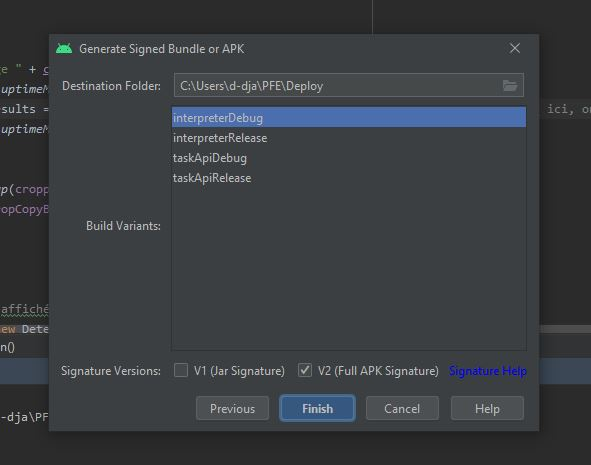
\includegraphics[width=0.7\textwidth]{images/generateAPK.jpg}
  \caption{Génération de l'APK}
  \label{fig:genapk}
\end{figure}

\section{Google Play Console}

Après avoir généré l'APK, nous pouvons désormais le déployer sur le Google Play. Pour cela, il faut disposer d'un compte Google Play Console \footnote{\url{https://play.google.com/console/about/}}. Une fois connecté sur la plateforme, il faut aller sur créer une application et suivre les instructions.

\begin{figure}[h!]
\centering
  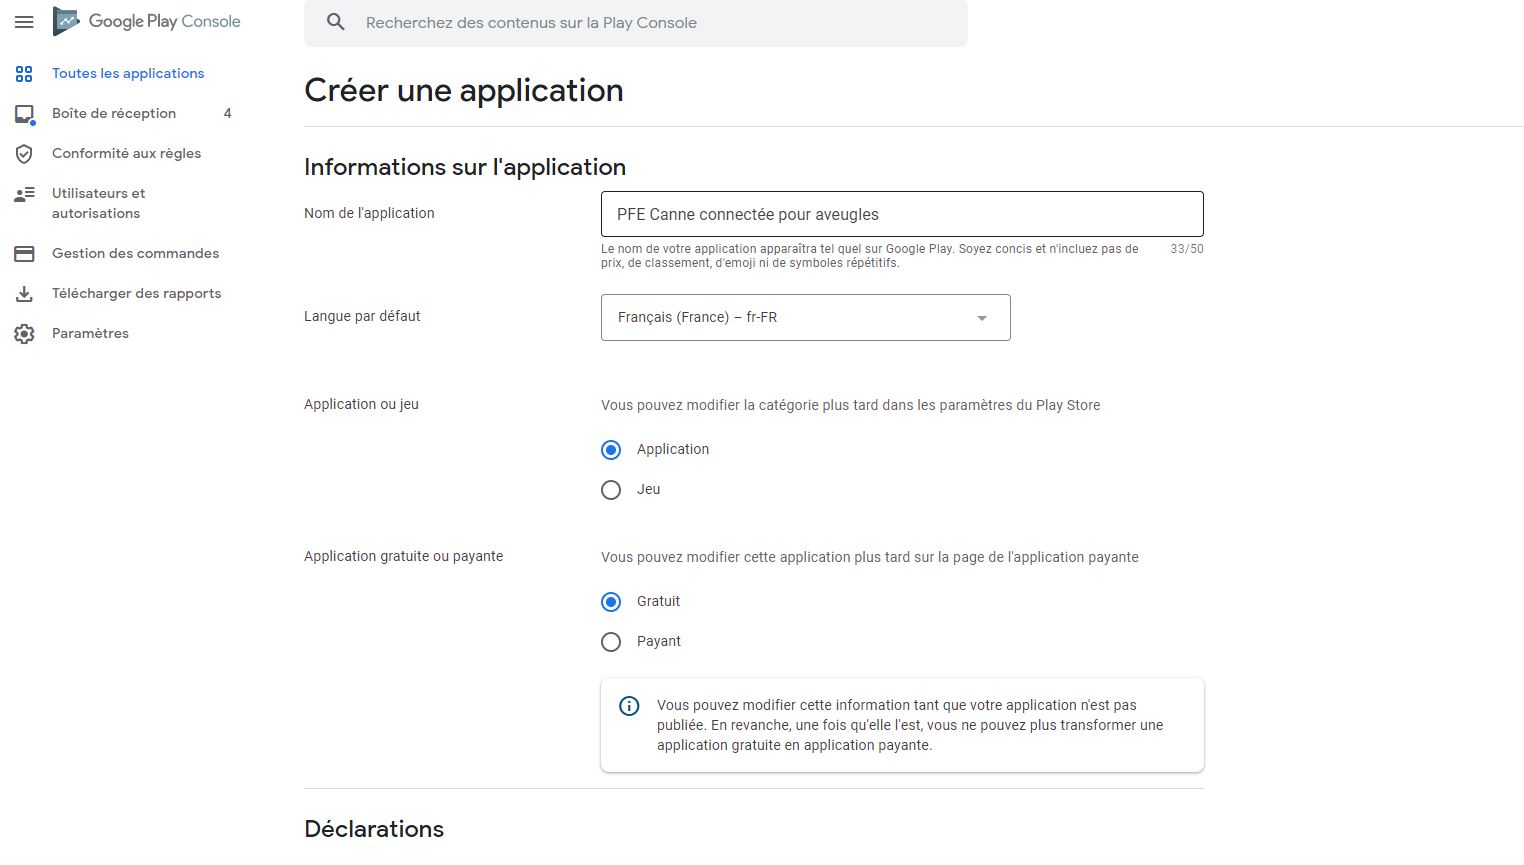
\includegraphics[width=1\textwidth]{images/CreateAppConsole.JPG}
  \caption{Creation de l'application sur Google Play Console}
  \label{fig:createappconsole}
\end{figure}

On attérrit sur une section avec des menus spécifique à l'application qu'on souhaite déployer. Il faut ensuite aller sur le menu Production puis déposer le fichier .apk généré précédemment.
\newpage

\begin{figure}[h!]
\centering
  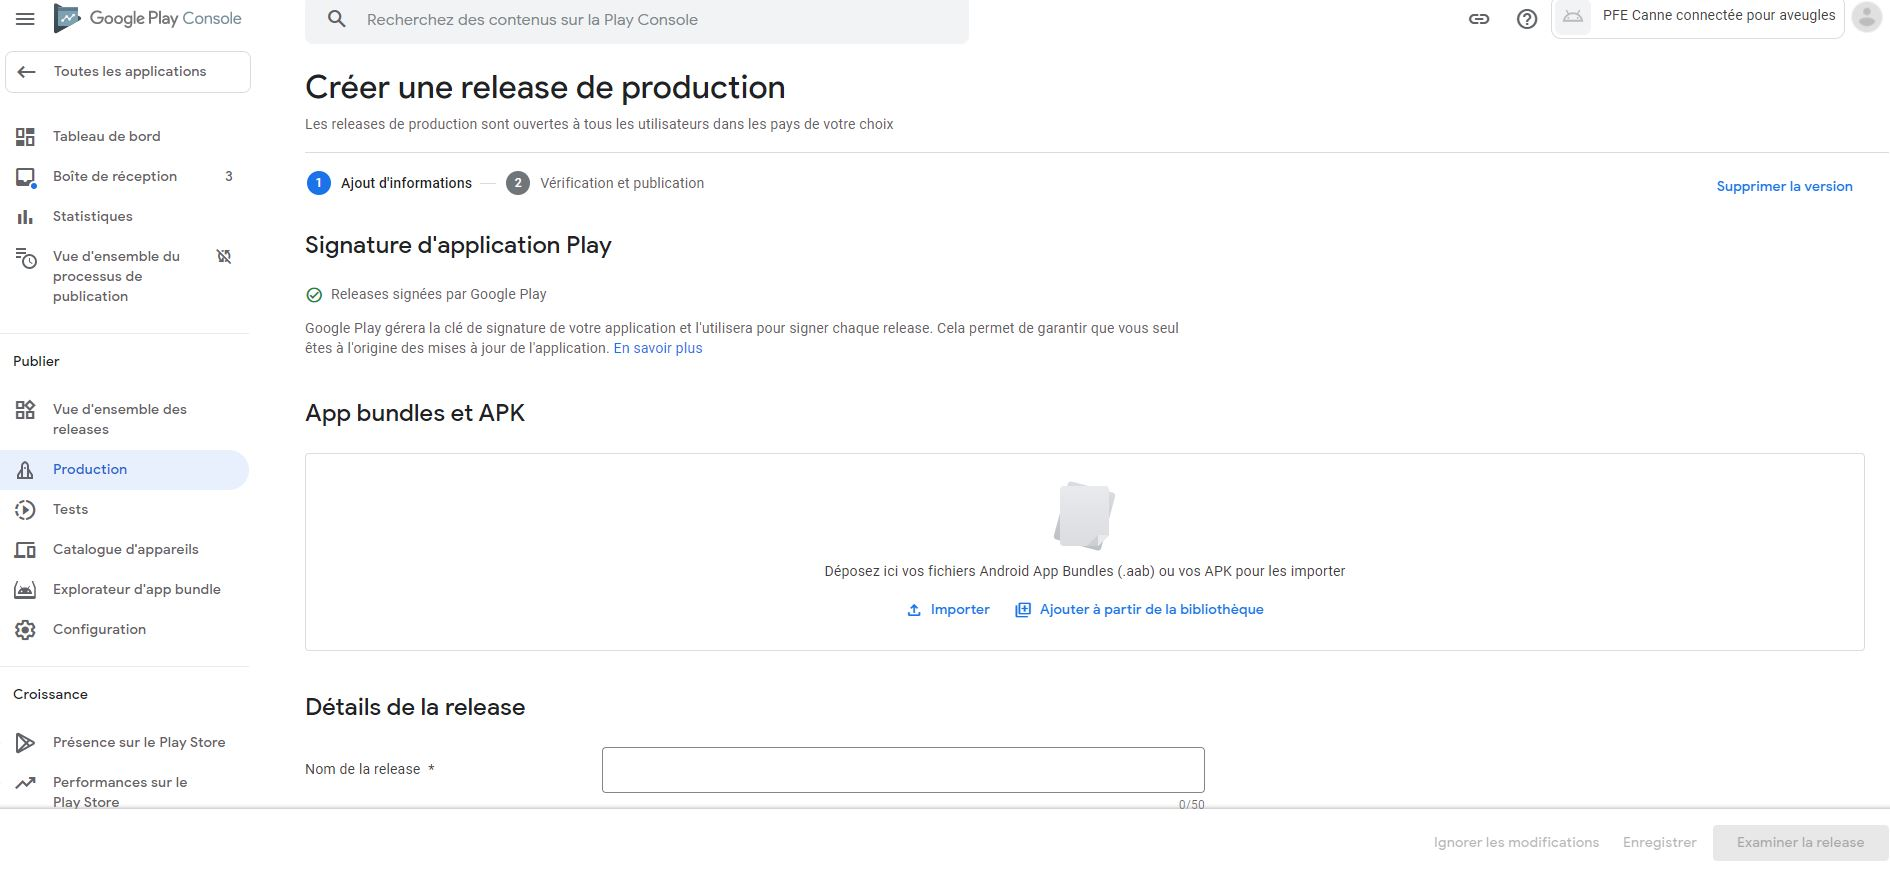
\includegraphics[width=1\textwidth]{images/release.JPG}
  \caption{Dépôt de l'APK sur Google Play Console}
  \label{fig:depotapk}
\end{figure}

Une fois effectué l'application ne sera pas encore disponible sur le Google Play, il faudra attendre que les vérifications soient terminées. Si l'application est conforme aux politiques de Google, il sera publié par la suite sur le Google Play.

\section{Vérification du déploiement}
La dernière étape du déploiement est la vérification de la disponibilité de l'application sur le Google Play. Pour cela, il suffit de se rendre sur le Google Play et rechercher le nom de l'application. L'application devrait apparaître parmis la liste des résultats de recherche.

\chapter{Installation}
\section{Installation depuis Google Play}
Pour installer l'application depuis le Goole Play, il suffit de l'installer comme n'importe quel autre application du Google Play. Ouvrir Google Play sur le smartphone sur lequel on souhaite installer l'application, rechercher le nom de l'application et installer l'application. \\
Une autre façon de faire serait d'utiliser directement Google Play avec le navigateur puis de sélectionner sur quel terminal on souhaite l'installer. Cette deuxième manière de faire sera plus pratique dans le cadre d'une installation sur une multitude d'appareils. \\
\begin{figure}[h!]
\centering
  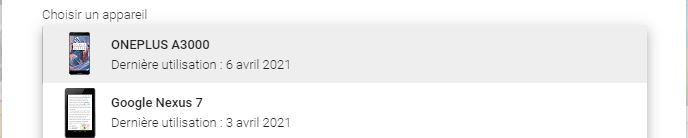
\includegraphics[width=0.7\textwidth]{images/DeviceChoice.JPG}
  \caption{Choix des appareils}
  \label{fig:devicechoice}
\end{figure}
\section{Installation à partir du fichier APK}
Pour installer l'application sans passer par le Google Play, il suffit de disposer du fichier .apk (voir  \nameref{genapk}). Transférer l'application sur le smartphone et avant de cliquer dessus pour l'installer, il faut autoriser l'installation d'application à partir de source inconnue. Cette option se trouve dans la partie « Sécurité » des paramètres du smartphone. Une fois cela fait, à l'aide d'un explorateur de fichier, naviguer jusqu'à l'emplacement du fichier .apk puis cliquer dessus pour l'installer.

\section{Installation depuis Android Studio}
Une dernière façon d'installer l'application est d'utiliser l'environnement de développement Android Studio. Pour cela, assurer vous d'avoir le code source et de vérifier que celui-ci compile bien. Ensuite, il faut connecter le smartphone à l'ordinateur et activer le déboggage usb dans les paramètres. Cette option est, comme son nom l’indique, pour les développeurs afin de déboguer une application. Il n'est donc pas recommandé d'utiliser cette méthode dans le cadre d'un déploiement en production. Cette option se trouve dans la partie "Option de développement" dans les paramètres du smartphone. Ensuite, sur Android Studio, il suffit de lancer l'application en sélectionnant le smartphone en tant que source et non l'émulateur de terminal Android.

\chapter{Configuration}
\section{vérification des configurations}
L'application n'a pas besoin d'être configuré pour être utilisé. Une fois installé sur le terminal, l'utilisateur peut directement s'en servir. En cas d'anomalies, vérifier :
\begin{itemize}
  \item La possibilité d'utiliser la caméra arrière du smartphone.
  \item La possibilité d'utiliser le haut-parleur du smartphone.
  \item Le mode du synthétiseur vocal (mode mute ou unmute)
  \item Le niveau du seuil de détection minimal
\end{itemize}

Ces éléments sont, en effet, indispensables pour que l'application puisse fonctionner correctement. Si l'anomalie persiste se rapprocher d'un développeur afin d'entamer une procédure de recherche plus approfondie.

\end{document}